\renewcommand{\NomeBloco}{\emph{vref\_block\_with\_mux}}
\renewcommand{\NomeBlocoA}{vrefblockwithmux}
\renewcommand{\NomePTab}{tab_\NomeBlocoA}
\renewcommand{\NomeSTab}{tab_\NomeBlocoA2}
\renewcommand{\NomePFig}{fig_\NomeBlocoA}
\renewcommand{\NomeSFig}{fig_\NomeBlocoA2}
\renewcommand{\NomeTTab}{tab_\NomeBlocoA3}

O bloco \NomeBloco{} tem a finalidade de selecionar a tens\~ao de refer\^encia a ser utilizada nos blocos de compara{\c c}\~ao do circuito, al\'em de retornar a tens\~ao de refer\^encia utilizada pelo bloco \emph{TIA}. A \autoref{\NomePTab} indica a Tabela Verdade do bloco. Embora tenha uma l\'ogica digital, o circuito permite sa\'idas anal\'ogicas.

\begin{table}[htbp]

\caption{Tabela Verdade do bloco \NomeBloco}%
\label{\NomePTab}
\centering
\begin{tabular}{ccccc}
    \toprule
    D0 & D1 & D2 & D3 & Out \\
    \midrule \midrule
    0 & 0 & 0 & 0 & Vref\_plus\\
    \midrule
    0 & 1 & 0 & 0 & Vref\\
    \midrule
    1 & 0 & 0 & 0 & Vref\_minus2\\
    \midrule
    1 & 1 & 0 & 0 & Vref\_minus3\\
    \midrule
    X & X & 0 & 1 & Vref\_minus4\\
    \midrule
    X & X & 1 & 0 & Vref\_minus5\\
    \midrule
    X & X & 1 & 1 & Vref\_minus6\\
\bottomrule

\end{tabular}
\fonte{Produzido pelo autor.}
\end{table}

O bloco apresenta as defini{\c c}\~oes de sinais de entrada e sa\'ida referidos na \autoref{\NomeSTab}.

\begin{table}[htbp]
\caption{Sinais do bloco \NomeBloco}
\label{\NomeSTab}
\centering
\begin{tabular}{ccl}

    \toprule
    Sinal & Tipo    & Descri{\c c}\~ao      \\
    \midrule \midrule
    D0   & Entrada   & Entrada de sele{\c c}\~ao 1 \\
    \midrule
    D1   & Entrada   & Entrada de sele{\c c}\~ao 2 \\
    \midrule
    D2   & Entrada   & Entrada de sele{\c c}\~ao 3 \\
    \midrule
    D3   & Entrada   & Entrada de sele{\c c}\~ao 4 \\
    \midrule
    Vref\_pixel   & Sa\'ida   & Tens\~ao de refer\^encia selecionada \\
    \midrule
    Vref\_clk¹  & Sa\'ida   & Tens\~ao de refer\^encia do Clock \\
    \midrule
    Vref\_comp²  & Sa\'ida   & Tens\~ao de refer\^encia do Clock do bloco teste \\
    \bottomrule
\end{tabular}
\legend{Fonte: Produzido pelo autor}
\legend{¹ Essa tens\~ao \'e igual \'a sa\'ida Vref\_minus do bloco \emph{vref\_block}\\² Essa tens\~ao \'e igual \'a sa\'ida Vref\_extra do bloco \emph{vref\_block}}
\end{table}

O circuito projetado para o bloco \'e demonstrado na \autoref{\NomePFig}.

\begin{figure}[htb]
 \label{NomePFig}
 \centering
    \centering
    \caption{Circuito CMOS projetado para o bloco \NomeBloco} \label{\NomePFig}
    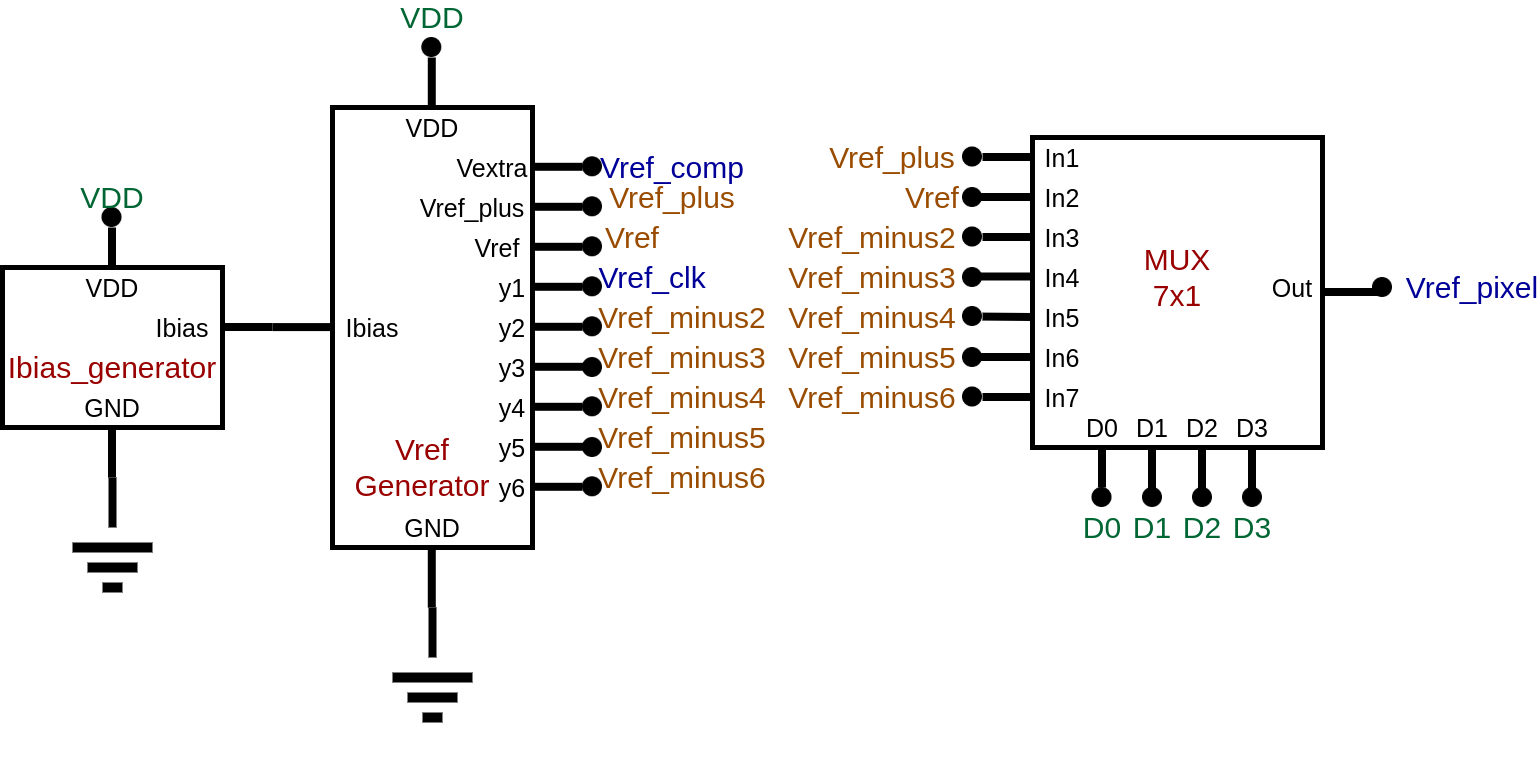
\includegraphics[scale=0.28]{Circuitos/vref_block.png}
    \legend{Fonte: Produzido pelo autor}
\end{figure}

\begin{figure}[htb]
 \label{NomeSFig}
 \centering
    \centering
    \caption{Representa{\c c}\~ao em bloco do \NomeBloco} \label{NomeSFig}
    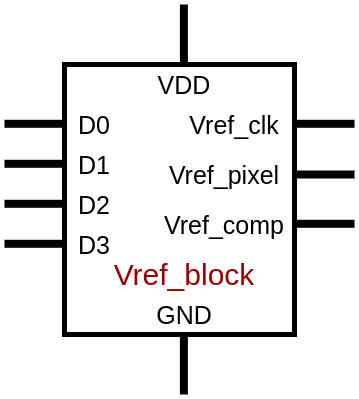
\includegraphics[scale=0.3]{Circuitos/vref_block_block.png}
    \legend{Fonte: Produzido pelo autor}
\end{figure}
